        \subsection{noise shaping}

	\begin{frame}\frametitle{sampling and quantization}\framesubtitle{Z-transform quick and dirty}
		\begin{table}
			\centering
%			\begin{footnotesize}
					\begin{tabular}{ccc}
					\hline
					\textbf{Z} &  & \textbf{time}\\
					\hline 
					$X(z)$ &$\leftrightarrow$& $x(n)$\\
					$X(z)\cdot z^{-k}$ &$\leftrightarrow$& $x(n-k)$\\
					\end{tabular}
%			\end{footnotesize}
		\end{table}
		\pause
		\textbf{transfer function}:
		\begin{equation}
			H(z) = \frac{out}{in} = \frac{Y(z)}{X(z)}
		\end{equation}
		\pause
		\textbf{spectrum}
		\begin{equation}
			H(\jOm) = H(z\big|_{z=e^{\jOm}})
		\end{equation}
	\end{frame}
	
	\begin{frame}\frametitle{sampling and quantization}\framesubtitle{noise shaping introduction}
		\textbf{idea}:
		\begin{itemize}
			\item	filter quantization error, shape its frequency response
			\pause
            \bigskip
			\item[$\Rightarrow$]	move power to high frequencies
			\item[$\Rightarrow$]	less recognizable in lower frequencies
		\end{itemize}
	\end{frame}
	
	\begin{frame}\frametitle{sampling and quantization}\framesubtitle{first order noise shaping 1/2}
       \begin{figure}[!hbt]
			\begin{center}
	            \begin{picture}(40,40)
	
	                %boxes
	                \put(27,17){\dashbox (11,20){}}
	                \put(19,3){\framebox (6,6){\scriptsize{$z^{-1}$}}}
	
	                %lines horizontal
	                \put(0,20){\vector(1,0){10}}
	                \put(15,20){\vector(1,0){15}}
	                \put(35,20){\vector(1,0){15}}
	                \put(25,12){\vector(1,0){5}}
	                \put(40,12){\vector(-1,0){5}}
	                
	                \put(32.5,6){\vector(-1,0){7.5}}
	                \put(19,6){\line(-1,0){6.5}}
	
	                %lines vertical
	                \put(25,20){\line(0,-1){8}}
	                \put(40,20){\line(0,-1){8}}
	                \put(12.5,6){\vector(0,1){11.5}}
	                \put(32.5,9.5){\line(0,-1){3.5}}
	                
	                \put(32.5,30){\vector(0,-1){7.5}}
	                
	                %circles
	                \put(12.5,20){\circle{5}} \put(11,19){{{+}}}
	                \put(32.5,20){\circle{5}} \put(31,19){{{+}}}
	                \put(32.5,12){\circle{5}} \put(31,11){{{+}}}
	                
	                \put(25,20){\circle*{1}}
	                \put(40,20){\circle*{1}}
	
	                %text
	                \put(29,12.5){\footnotesize{\shortstack[c]{-}}}
	                \put(14,16){\footnotesize{\shortstack[c]{-}}}
	                \put(25,38){\footnotesize{\shortstack[c]{Quantization}}}
	                \put(30,32){\footnotesize{\shortstack[c]{q(n)}}}
	                \put(0,22){\footnotesize{\shortstack[c]{x(n)}}}
	                \put(50,22){\footnotesize{\shortstack[c]{y(n)}}}
	
	            \end{picture}
			\end{center}
	    \end{figure}
	    \pause
		\begin{eqnarray}
			y(i) &=& [x(i)-q(i-1)]_Q \nonumber\\
			\pause
			&=& x(i)-q(i-1)+q(i)
		\end{eqnarray}
	\end{frame}
	
	\begin{frame}\frametitle{sampling and quantization}\framesubtitle{first order noise shaping 2/2}
		\begin{eqnarray}
			y(i) &=& x(i)-q(i-1)+q(n)\nonumber\\
			\pause
			Y(z) &=& X(z) - z^{-1}\cdot Q(z) + Q(z)\nonumber\\
			&=& X(z) + \only<3->{\textcolor{gtgold}}{\underbrace{(1-z^{-1})}_{H_\mathrm{Q}(z)}}\cdot Q(z)\\
			\pause
			\Rightarrow&&\nonumber\\
			H_\mathrm{Q}(z) &=& 1-z^{-1}\\
			\pause
            \bigskip
			|H_\mathrm{Q}(\jOm)| &=& |1-e^{-\jOm}|\\
			\pause
            \bigskip
			&=& 2\cdot \sin\left(\frac{\Omega}{2}\right) 
		\end{eqnarray}
	
	\end{frame}
	
	\begin{frame}\frametitle{sampling and quantization}\framesubtitle{second order noise shaping 1/2}
        \begin{figure}[!hbt]
			\begin{center}
	            \begin{picture}(40,40)
	
	                %boxes
	                \put(27,17){\dashbox (11,20){}}
	                \put(24,4){\framebox (6,4){\scriptsize{$z^{-1}$}}}
	                \put(24,-2){\framebox (6,4){\scriptsize{$z^{-2}$}}}
	
	                %lines horizontal
	                \put(0,20){\vector(1,0){10}}
	                \put(15,20){\vector(1,0){15}}
	                \put(35,20){\vector(1,0){15}}
	                \put(25,12){\vector(1,0){5}}
	                \put(40,12){\vector(-1,0){5}}
	                
	                \put(32.5,6){\vector(-1,0){2.5}}
	                \put(32.5,0){\vector(-1,0){2.5}}
	                
	                \put(24,6){\vector(-1,0){4}}
	                \put(24,0){\vector(-1,0){4}}
	                
	                \put(18,6){\vector(-1,0){3}}
	                \put(18,0){\line(-1,0){5.5}}
	
	                %lines vertical
	                \put(25,20){\line(0,-1){8}}
	                \put(40,20){\line(0,-1){8}}
	                \put(12.5,8.5){\vector(0,1){9}}
	                \put(32.5,9.5){\line(0,-1){9.5}}
	                
	                \put(32.5,30){\vector(0,-1){7.5}}

	                \put(12.5,0){\vector(0,1){3.5}}
	                
	                \put(12.5,19){$\oplus$}
	                \put(32.5,19){$\oplus$}
	                \put(32.5,11){$\oplus$}
	                \put(12.5,5){$\oplus$}
	                \put(17,5){$\otimes$}
	                \put(17,-1){$\otimes$}
	                %circles
	                %\put(12.5,20){\circle{5}} \put(11,19){{{+}}}
	                %\put(32.5,20){\circle{5}} \put(31,19){{{+}}}
	                %\put(32.5,12){\circle{5}} \put(31,11){{{+}}}
	                %\put(12.5,6){\circle{5}} \put(11,5){{{+}}}
	                %\put(19,6){\circle{2}} \put(18,5){{{x}}}
	                %\put(19,0){\circle{2}} \put(18,-1){{{x}}}
	                
	                \put(25,20){\circle*{1}}
	                \put(40,20){\circle*{1}}
	                \put(32.5,6){\circle*{1}}
	
	                %text
	                \put(29,12.5){\footnotesize{\shortstack[c]{-}}}
	                \put(14,16){\footnotesize{\shortstack[c]{-}}}
	                \put(25,38){\footnotesize{\shortstack[c]{Quantizer}}}
	                \put(30,32){\footnotesize{\shortstack[c]{q(n)}}}
	                \put(0,22){\footnotesize{\shortstack[c]{x(n)}}}
	                \put(50,22){\footnotesize{\shortstack[c]{y(n)}}}
	                \put(19.5,7){\footnotesize{\shortstack[c]{2}}}
	                \put(19,1){\footnotesize{\shortstack[c]{-1}}}
	
	            \end{picture}
			\end{center}
	    \end{figure}
	    \pause
		\begin{eqnarray}
			y(n) &=& [x(n)-2\cdot q(n-1) + q(n-2)]_Q \nonumber\\
			\pause
			&=& x(n)-2\cdot q(n-1)+q(n-2)+q(n)
		\end{eqnarray}
	\end{frame}
	
	\begin{frame}\frametitle{sampling and quantization}\framesubtitle{second order noise shaping 2/2}
		\begin{eqnarray}
			y(n) &=& x(n)-2\cdot q(n-1)+q(n-2)+q(n)\nonumber\\
			\pause
			Y(z) &=& X(z) - 2\cdot z^{-1}\cdot Q(z) + z^{-2}\cdot Q(z) + Q(z)\nonumber\\
			&=& X(z) + \only<3->{\textcolor{gtgold}}{(1-z^{-1})^2}\cdot Q(z)\\
			\pause
			\Rightarrow&&\nonumber\\
			H_\mathrm{Q}(z) &=& (1-z^{-1})^2
		\end{eqnarray}
		\pause
		without derivation: nth order noise shaping
			\begin{eqnarray}
				Y(z) &=& X(z) + (1-z^{-1})^n\cdot Q(z)\\
			\Rightarrow&&\nonumber\\
			H_\mathrm{Q}(z) &=& (1-z^{-1})^n
			\end{eqnarray}
	\end{frame}
	
	\begin{frame}\frametitle{sampling and quantization}\framesubtitle{higher order noise shaping}
		\begin{figure}
			\centering
				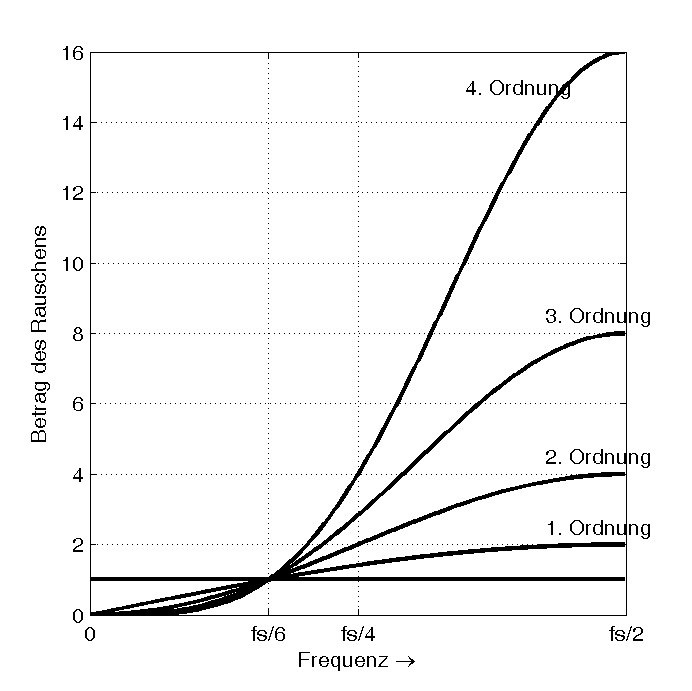
\includegraphics[scale=0.6]{Graph/noiseshaping}
		\end{figure}
	\end{frame}
	
	\begin{frame}\frametitle{sampling and quantization}\framesubtitle{arbitrary noise shaping transfer functions}
		\begin{figure}
			\centering
				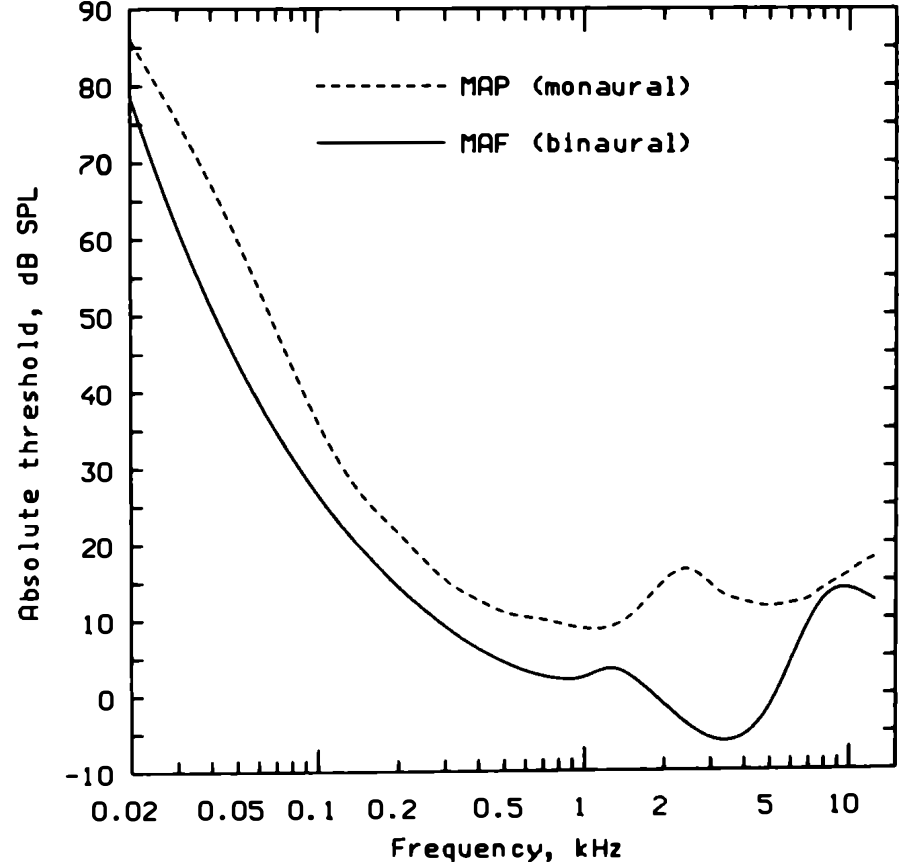
\includegraphics[scale=0.3]{Graph/ATH}
		\end{figure}
	\end{frame}
	
	\begin{frame}\frametitle{sampling and quantization}\framesubtitle{dither \& noise shaping 1/3}
        \begin{figure}[!hbt]
			\begin{center}
	            \begin{picture}(120,40)
	
	                %boxes
	                \put(27,17){\dashbox (11,20){}}
	                \put(19,3){\framebox (6,6){\scriptsize{$z^{-1}$}}}
	
	                %lines horizontal
	                \put(0,20){\vector(1,0){10}}
	                \put(15,20){\vector(1,0){15}}
	                \put(35,20){\vector(1,0){15}}
	                \put(25,12){\vector(1,0){5}}
	                \put(40,12){\vector(-1,0){5}}
	                
	                \put(32.5,6){\vector(-1,0){7.5}}
	                \put(19,6){\line(-1,0){6.5}}
	
	                %lines vertical
	                \put(25,20){\line(0,-1){8}}
	                \put(40,20){\line(0,-1){8}}
	                \put(12.5,6){\vector(0,1){11.5}}
	                \put(32.5,9.5){\line(0,-1){3.5}}
	                
	                \put(32.5,30){\vector(0,-1){7.5}}

	                \put(12.5,30){\vector(0,-1){7.5}}
	                
	                %circles
	                \put(12.5,20){\circle{5}} \put(11,19){{{+}}}
	                \put(32.5,20){\circle{5}} \put(31,19){{{+}}}
	                \put(32.5,12){\circle{5}} \put(31,11){{{+}}}
	                
	                \put(25,20){\circle*{1}}
	                \put(40,20){\circle*{1}}
	
	                %text
	                \put(29,12.5){\footnotesize{\shortstack[c]{-}}}
	                \put(14,16){\footnotesize{\shortstack[c]{-}}}
	                \put(25,38){\footnotesize{\shortstack[c]{Quantizer}}}
	                \put(30,32){\footnotesize{\shortstack[c]{q(n)}}}
	                \put(0,22){\footnotesize{\shortstack[c]{x(n)}}}
	                \put(50,22){\footnotesize{\shortstack[c]{y(n)}}}
	                \put(10,32){\footnotesize{\shortstack[c]{d(n)}}}

	                \put(20,-5){\footnotesize{\shortstack[c]{System A}}}







	
	                %boxes
	                \put(87,17){\dashbox (11,20){}}
	                \put(79,3){\framebox (6,6){\scriptsize{$z^{-1}$}}}
	
	                %lines horizontal
	                \put(60,20){\vector(1,0){10}}
	                \put(75,20){\vector(1,0){5}}
	                \put(85,20){\vector(1,0){5}}
	                \put(95,20){\vector(1,0){15}}
	                \put(77.5,12){\vector(1,0){12.5}}
	                \put(100,12){\vector(-1,0){5}}
	                
	                \put(92.5,6){\vector(-1,0){7.5}}
	                \put(79,6){\line(-1,0){6.5}}
	
	                %lines vertical
	                \put(77.5,20){\line(0,-1){8}}
	                \put(100,20){\line(0,-1){8}}
	                \put(72.5,6){\vector(0,1){11.5}}
	                \put(92.5,9.5){\line(0,-1){3.5}}
	                
	                \put(92.5,30){\vector(0,-1){7.5}}

	                \put(82.5,30){\vector(0,-1){7.5}}
	                
	                %circles
	                \put(72.5,20){\circle{5}} \put(71,19){{{+}}}
	                \put(82.5,20){\circle{5}} \put(81,19){{{+}}}
	                \put(92.5,20){\circle{5}} \put(91,19){{{+}}}
	                \put(92.5,12){\circle{5}} \put(91,11){{{+}}}
	                
	                \put(77.5,20){\circle*{1}}
	                \put(100,20){\circle*{1}}
	
	                %text
	                \put(89,12.5){\footnotesize{\shortstack[c]{-}}}
	                \put(74,16){\footnotesize{\shortstack[c]{-}}}
	                \put(85,38){\footnotesize{\shortstack[c]{Quantizer}}}
	                \put(90,32){\footnotesize{\shortstack[c]{q(n)}}}
	                \put(60,22){\footnotesize{\shortstack[c]{x(n)}}}
	                \put(110,22){\footnotesize{\shortstack[c]{y(n)}}}
	                \put(80,32){\footnotesize{\shortstack[c]{d(n)}}}
	                
	                \put(80,-5){\footnotesize{\shortstack[c]{System B}}}
	
	            \end{picture}
			\end{center}
	    \end{figure}
	\end{frame}
	
	\begin{frame}\frametitle{sampling and quantization}\framesubtitle{dither \& noise shaping 2/3}
		System A
			\begin{eqnarray}
				y(n) &=& [x(n) + d(n) -q(n-1)]_Q \nonumber\\
				&=& x(n)+d(n)-q(n-1)+q(n)
			\end{eqnarray}
			\pause
			\begin{eqnarray}
				Y(z) &=& X(z) - z^{-1}\cdot Q(z) + Q(z) + D(z)\nonumber\\
				&=& X(z) + (1-z^{-1})\cdot Q(z) + D(z)
			\end{eqnarray}
	\end{frame}
	
	\begin{frame}\frametitle{sampling and quantization}\framesubtitle{dither \& noise shaping 3/3}
		System B
			\begin{eqnarray}
				y(n) &=& [x(n) + d(n) - q(n-1) - d(n-1)]_Q \nonumber\\
				&=& x(n)-q(n-1)+q(n)-d(n-1)+d(n)
			\end{eqnarray}
			\pause
			\begin{eqnarray}
				Y(z) &=& X(z) - z^{-1}\cdot Q(z) + Q(z) - z^{-1}\cdot D(z) + D(z)\nonumber\\
				&=& X(z) + (1-z^{-1})\cdot (Q(z) + D(z))
			\end{eqnarray}
	\end{frame}
	
	\begin{frame}\frametitle{sampling and quantization}\framesubtitle{noise shaping audio examples}
        \begin{itemize}
            \item   \unit[16]{bit}: \includeaudio{audio/00_Master_16_bit.mp3}
            \item   \unit[8]{bit}: \includeaudio{audio/01_Truncate_8_bit.mp3}
            \item   \unit[8]{bit} dither: \includeaudio{audio/02_Standard_Dither_8_bit.mp3}
            \item   \unit[8]{bit} standard noise shaping: \includeaudio{audio/03_Most_Widely_Known_8_bit.mp3}
            \item   \unit[8]{bit} powerful noise shaping: \includeaudio{audio/04_Most_Powerful_8_bit.mp3}
        \end{itemize}
	\end{frame}
	
	\begin{frame}\frametitle{sampling and quantization}\framesubtitle{noise shaping spectrograms}
		\begin{figure}
			\centering
				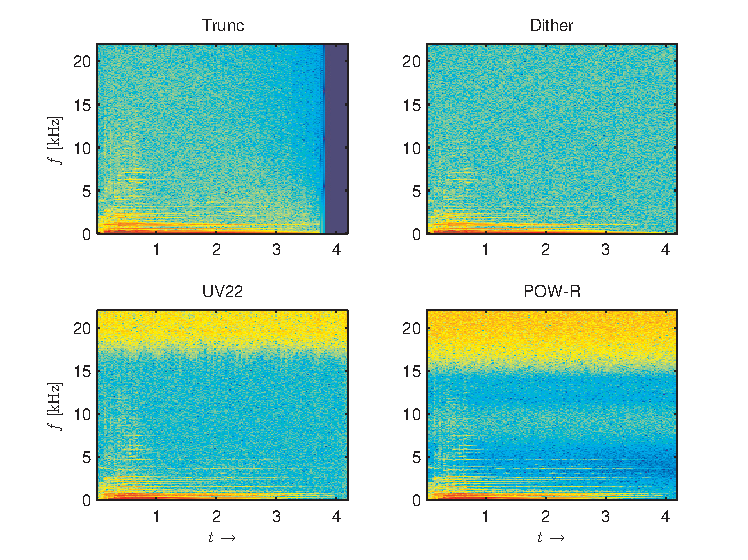
\includegraphics[scale=0.8]{Graph/noiseshaping_spectrum}
		\end{figure}
	\end{frame}
	
			        		

